\documentclass[letterpaper,10pt]{article}

\usepackage{geometry}
\usepackage{enumitem}
\usepackage{hyperref}
\usepackage{blindtext}
% \usepackage[dvipsnames]{xcolor}
\usepackage[table, rgb, svgnames, dvipsnames, rgba]{xcolor}
% \usepackage[default]{lato}
% % \usepackage[default]{roboto}
% \usepackage[T1]{fontenc}
\usepackage{tabularx}
\usepackage{array}
\usepackage{graphicx}
\usepackage{svg}


\pagestyle{empty}
\geometry{margin=.75in}
\setlength{\parindent}{0pt}
% \setlength{\parskip}{0.5em}


\title{Optimal path planning for an odor tracking robot}
\author{Tamzeed Elahi Toha}
\date{\today}



\begin{document}
\maketitle

\section*{Problem Statement}
Odor tracking problem fundamentally involves finding the source of an odor and tracking the odor plume in a way that ensures further odor encounter. In my algorithm, the source estimation is done by a deconvolution algorithm. To solve the second part of the problem I will use the optimal control theory in accordance with the course curriculum. There might be two approaches to solve this problem. In both of them we try to find a optimal path that maximizes the probability of encountering the odor while minimizing the path length. The first approach can be to use wind dynamics as constraints with fixed end points. And, the second approach can be to give the agent some dynamics and constraining it with some curve $f(x,y) = 0$ where $f(x,y)$ is derived from the wind dynamics. The next challenge would be to come up with the cost function that we have to optimize. Although this course mostly focuses on linear systems, and the problem is non-linear, I will try to incorporate linearization techniques or numerical methods to solve the problem.

% 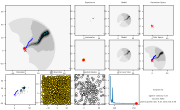
\includegraphics[width=\textwidth]{images/odor_tracking_summary.png}
\includesvg[width=\textwidth]{images/odor_tracking_summary.svg}

\section*{Introduction}

\end{document}